%\subsection{Технический аспект}
\begin{frame}{Технические шаги для решения задачи}
Для решения содержательных задач необходимо реализовать ряд вспомогательных функций:
\begin{itemize}
\item определить соответствие хода правилам;
\item строить траектории на пустой доске;
\item оценивать последовательность взятий и величину размена на поле;
\item находить фигуры, способные повлиять на размен, и позиции, которые им необходимо занять;
\end{itemize}
Все эти функции были реализованы.
%построение цепочки
\end{frame}

\begin{frame}{Пример цепочки: дерево (повтор)}
\begin{tabular}{ll}
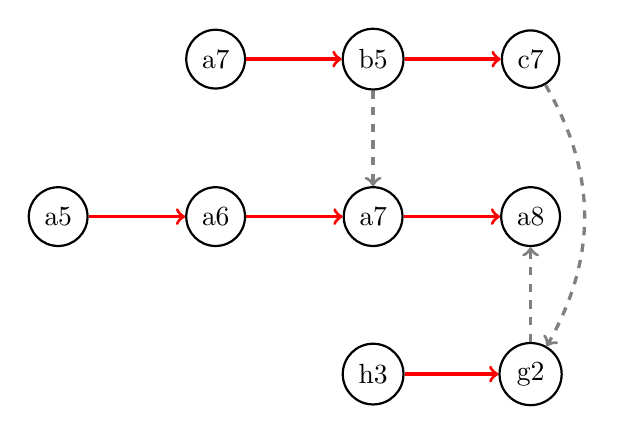
\begin{tikzpicture}
\begin{scope}[every node/.style={circle,thick,draw}]
    \node (A5) at (0,0) {a5};
    \node (A6) at (2,0) {a6};
    \node (A7) at (4,0) {a7};
    \node (A8) at (6,0) {a8};
    \node (NA7) at (2,2) {a7};
    \node (B5) at (4,2) {b5};
    \node (C7) at (6,2) {c7};
    \node (H3) at (4,-2) {h3};
    \node (G2) at (6,-2) {g2};
\end{scope}

\begin{scope}[%>={Stealth[black]},
              every node/.style={fill=white,circle},
              every edge/.style={draw=red,very thick}]
    % подцепочка 0
    \path [->] (A5) edge (A6);
    \path [->] (A6) edge (A7);
    \path [->] (A7) edge (A8);
    % Защита
    \path [->] (H3) edge (G2);
    \path [->] (G2) edge[gray, draw=gray, dashed] (A8);
    % Отступление 
    \path [->] (NA7) edge (B5);
    \path [->] (B5) edge (C7);
    \path [->] (B5) edge[gray, draw=gray, dashed] (A7);
    \path [->] (C7) edge[gray, draw=gray, dashed, bend left] (G2);
    %\path [->] (B) edge[bend right=60] node {$1$} (E); 
\end{scope}
\end{tikzpicture}
&
{\scalebox{0.5}{\showDiagram{Pa5, Na7, bh3}{}}}
\end{tabular}

Пунктиром отмечены поля, к которым <<подтянуты>> соотвествующие подцепочки.
\end{frame}

\begin{frame}{Формальная модель}
Множество полей доски $\mathcal{S} \coloneqq \{a1, b1, \dots, h8\}$.\\
Типы полей $\mathcal{ST} \coloneqq \{stop, internal\}$ --- поля остановки или промежуточные.\\
Множество типов фигур $\mathcal{K} \coloneqq \{ K, Q, R, B, N, P \}$ \\
Цвета соперников $\mathcal{C} \coloneqq \{black, white\}$ \\
Траектория $\mathcal{T} \in \left( \mathcal{S} \times \mathcal{ST} \right)^+$ --- упорядоченный набор полей.\\
Доска $\Delta  \colon \mathcal{S} \to \mathcal{K} \times \mathcal{C} $ --- соответсвтие полю фигуры (типа и цвета). \\
Цепочка $Chain \coloneqq \langle color, traj, sa \rangle$,  где $color \in \mathcal{C}$ --  цвет цепочки, $traj \in \mathcal{T}$ -- основная траектория цепочки, $sa \subset \mathbb{N} \times 2^{\mathtt{Chains}}$ -- множество вспомогательных действий для проходимости поля траектории. \\
В этом контексте понятие фигуры принимает вид всех цепочек одного цвета с общим началом траекторий.
\end{frame}

%картинка фигуры =_=
\begin{frame}{Пример фигуры}
\begin{tabular}{ll}
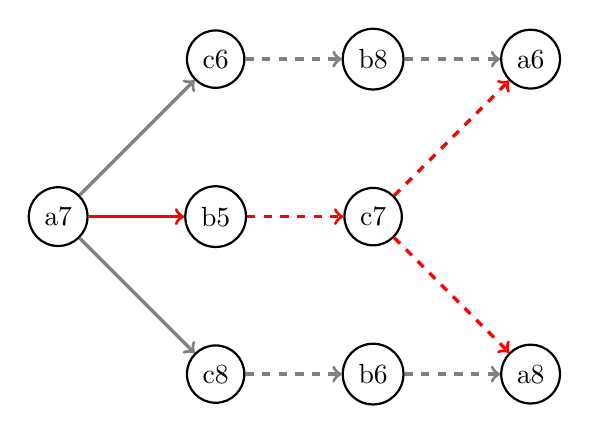
\begin{tikzpicture}
\begin{scope}[every node/.style={circle,thick,draw}]
    \node (A7) at (0,0) {a7};
    \node (B5) at (2,0) {b5};
    \node (C7) at (4,0) {c7};
    \node (B6) at (4,-2) {b6};
    \node (B8) at (4,2) {b8};
    \node (A6) at (6,2) {a6};
    \node (A8) at (6,-2) {a8};
    \node (C6) at (2,2) {c6};
    \node (C8) at (2,-2) {c8};
\end{scope}

\begin{scope}[%>={Stealth[black]},
              every node/.style={fill=white,circle},
              every edge/.style={draw=red,very thick}]
    % подцепочка 0
    \path [->] (A7) edge (B5);
    \path [->] (B5) edge[red, draw=red, dashed] (C7);
    \path [->] (C7) edge[red, draw=red, dashed] (A6);
    \path [->] (C7) edge[red, draw=red, dashed] (A8);
    % Защита
    \path [->] (A7) edge[gray, draw=gray] (C6);
    \path [->] (C6) edge[gray, draw=gray, dashed] (B8);
    \path [->] (B8) edge[gray, draw=gray, dashed] (A6);
    \path [->] (A7) edge[gray, draw=gray] (C8);
    \path [->] (C8) edge[gray, draw=gray, dashed] (B6);
    \path [->] (B6) edge[gray, draw=gray, dashed] (A8);
    %\path [->] (B) edge[bend right=60] node {$1$} (E); 
\end{scope}
\end{tikzpicture}
&
{\scalebox{0.5}{\showDiagram{Pa5, Na7, bh3}{}}}
\end{tabular}

Пунктиром отмечены цепочки, <<поддерживающие>> размен.
\end{frame}

\endinput
\begin{frame}{Формализация: построение цепи}
\begin{columns}
\column{0.5\textwidth}
\begin{figure}
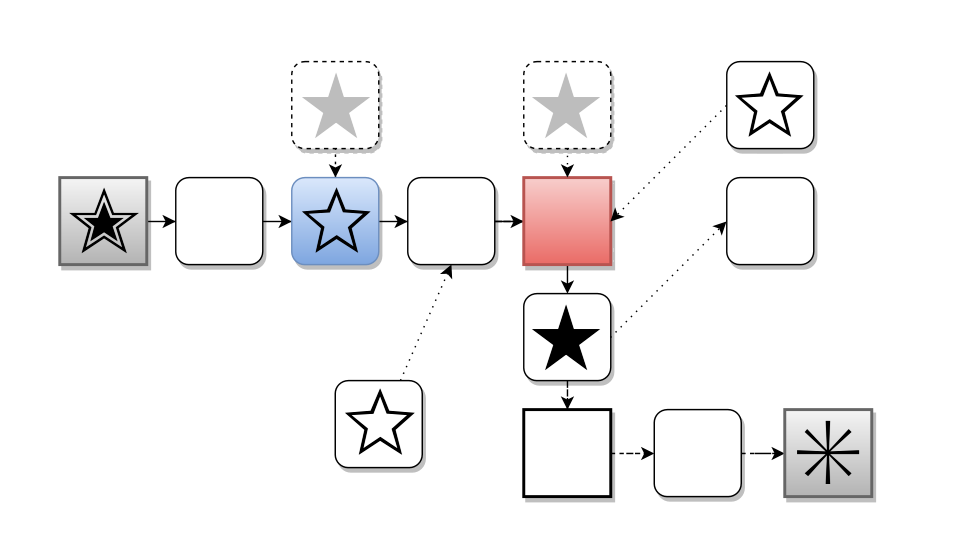
\includegraphics[scale=0.2]{./pictures/chain.png}
\end{figure}
\column{0.5\textwidth}
\begin{itemize}
\item определение цели для фигуры
\item построение траектории - подцепи-0
\item определение проходимости траектории
\item построение подцепей высших порядков
\end{itemize}
\end{columns}
Так как цепи весьма вариативны, необходимо выбрать оптимальное поддерево подцепей для цепи - произвести локальную оптимизацию.
\end{frame}

\begin{frame}{Формализация: оптимизация при построении}
\begin{columns}
\column{0.5\textwidth}
\begin{figure}
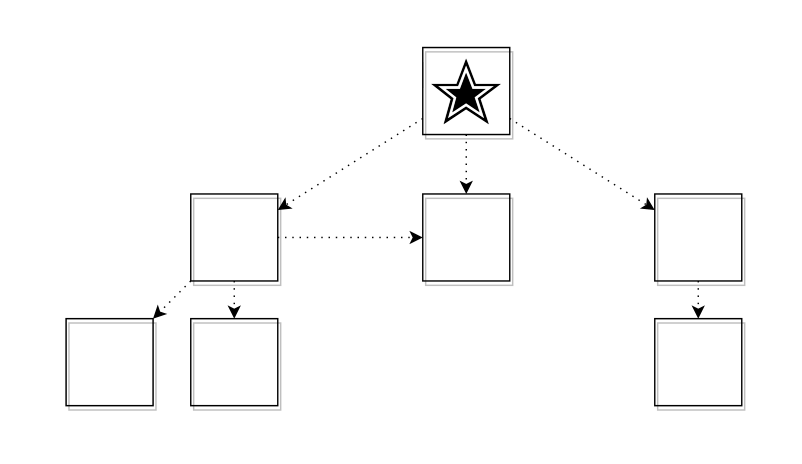
\includegraphics[scale=0.2]{./pictures/piece.png}
\end{figure}
\column{0.5\textwidth}
\begin{itemize}
\item квадраты - поля доски
\item с каждым полем связаны цепи
\item количество и качество цепей влияет на вес хода
\end{itemize}
\end{columns}
Глобальная оптимизация заключается в уточнении оценки для фигур по числу цепей, что может повлиять на уже построенные цепи
\end{frame}

